\documentclass[twocolumn,conference]{article}

\usepackage{amsmath,amssymb,amsfonts}
\usepackage{xcolor}
\usepackage{listings}
\usepackage{inputenc}
\usepackage{graphicx}
\usepackage{authblk}
\usepackage{enumerate}
\usepackage{caption}

\usepackage{array,booktabs,longtable,tabularx}
\usepackage{ltablex}
\usepackage{wrapfig,lipsum,booktabs}
\usepackage{multirow}

\providecommand{\keywords}[1]
{
  \small	
  \textbf{\textit{Keywords---}} #1
}

\begin{document}
\author[1]{Eric Raphael Huiza Pereyra}
\affil[1]{Pontifical Catholic University of Peru}
\affil[]{\textit{eric.huiza@pucp.edu.pe}}

\author[2]{Cesar Augusto Olivares Poggi}
\affil[2]{Pontifical Catholic University of Peru}
\affil[]{\textit{cesar.olivares@pucp.edu.pe}}

\title{%
	\vspace{-2.0cm}
	\textbf{Talking with signs} \\	
	\Large \textbf{A simple method to detect nouns and numbers in a non-annotated signs language corpus}
}

\maketitle
    
\begin{abstract}
People with deafness or hearing disabilities who aim to use computer based systems rely on state-of-art video classification and human action recognition techniques that combine traditional movement pattern recognition and deep learning techniques. In this work we present a pipeline for semi-automatic video annotation applied to a non-annotated \textit{Peruvian Signs Language} (PSL) corpus along with a novel method for a progressive detection of PSL elements (nSDm). We produced a set of video annotations indicating signs appearances for a small set of nouns and numbers along with a \textit{labeled PSL dataset} (PSL dataset). A composite model obtained from the combination of a 2D CNN trained with movement patterns extracted from the PSL dataset using Lucas Kanade optical flow, and a RNN with LSTM cells trained with raw rgb frames extracted from the PSL dataset achieved 0.5994 AUC for the Precision-Recall curve on signs classification tasks, reporting state-of-art results over the PSL dataset. \\
\keywords{Video Classification, Human Actions Detection, Peruvian Signs Language, Optical Flow, 2D CNN, LSTM.}
\end{abstract}

\section{Introduction}\label{intro}
The World Health Organization (WHO) stated that 466 million people world wide have disabling hearing loss, estimating that by 2050 over 900 million people will have disabling hearing loss that will represent a global cost of 750 million dollars annually \cite{deafness_and_hearing_loss_2019}. 

The Peruvian Institute of Informatics and Statistics (INEI) conducted a national disabilities survey with the objective of segmenting and acquiring a better understanding about disabilities that affect the Peruvian population \cite{disabilities_survey_2012}. Results showed that 1.8\% of the Peruvian population suffer at least partial when not permanent deafness or hearing limitations. 

Peruvians with deafness or hearing limitations use the Peruvian Signs Language (PSL) as their main communication medium. PSL is of mandatory usage at universities and certain public institutions, henceforth the importance of designing systems that are capable to support PSL inputs and outputs. Furthermore, in the same way as spoken languages, signs languages also present local variations e.g. people who live in Lima metropolitan area are not expected to use the same set of signs as people in other parts of the territory. This work uses the PSL variation used in Lima due to the difficulty or inability to find datasets for other PSL variations. 

\textit{The Grammar and Signs research group of the Pontifical Catholic University of Peru (PUCP)} built the first PSL corpus \cite{lsp_dataset} which is publicly available at the university digital archives. It is important to highlight that the corpus is neither labeled or annotated and cannot be used as it is for training or testing a model.

In this work we are approaching signs detection as a supervised learning task. Supervised learning requires labeled datasets to achieve satisfactory results during training and inference tasks. At the time of writing this work there were no labeled datasets available for PSL \cite{lsp_2015}. It configures a gap that could prevent or hinder research work on Human-Computer-Interaction at the Peruvian or Latin American space.

Current advances in Computer Vision (CV) and Natural Language Processing (NLP) make it possible to conceive systems that are capable of detecting and transcribing elements of sign languages thereby improving systems accessibility for people with physical limitations. This work reports results of a research conducted with the goal of producing a labeled PSL dataset for a set of signs limited to nouns and numbers as well as a novel method for detecting PSL signs by answering the following research questions:

\begin{enumerate}[(i)]
\item What are the currently available techniques for producing a labeled dataset for a set of signs limited to nouns and number from the non-annotated PSL corpus?\label{q1}
\item What are most relevant and currently available techniques for training a model with the labeled dataset described in the question above for detecting PSL nouns and numbers?\label{q2}
\item How precise and exhaustive is the model described in the above question on the detection of PSL nouns and numbers?\label{q3}
\end{enumerate}

This work has the main objective of producing a simple method that can be used as a baseline for other researchers interested on studying signs language and their different applications on the Human-Computer-Interaction field, we believe this work will produce a positive impact on the artificial intelligence community towards an increase in the number of research works using PSL which can contribute to increasing the number of people with deafness or hearing disabilities that can use computer based systems. We have divided this work main objective into following specific objectives for better traceability:

\begin{enumerate}[(i)]
\item Produce a labeled PSL dataset limited to nouns and numbers\label{o1}
\item Design and train a novel signs detection model (nSDm) for detecting signs at the labeled PSL dataset\label{o2}
\item Determine what is the performance of nSDm in terms of precision and recall\label{o3}
\end{enumerate}

The rest of the article is organized as follows. In section \ref{relatedwork} we review the related work on video classification for human actions recognition using network architectures that combine CNNs, 3D CNNs and movement patterns  for better features learning, we also review state-of-art pose estimation techniques. In section \ref{method} we introduce nSDm describing its design and architecture. In section \ref{experimentation} we evaluate nSDm precision and recall and answer research questions \ref{q1},\ref{q2},\ref{q3}. In section \ref{datasetdesc} we describe the PSL dataset produced at PUCP. In section \ref{videoannot} we describe the video annotation and data pre-processing techniques applied to produce the labeled PSL dataset and finally in section \ref{conclusion} we present our conclusions and future work.
\section{Related Work} \label{relatedwork}
\subsection{Action Recognition}
Human action recognition is an extensively studied field. Action recognition dataset like UCF101, HMDB51, THUMOS14  are available, researches tried to solve the human action recognition problem using different approaches including Optical Flow and 3D CNN \cite{qiu2017learning}.

\textbf{Optical Flow,} is defined as the pattern obtained from the motion of objects, surfaces and edges in a visual scene caused by the relative motion between the observer and a scene. It is computed by distributing movement velocities and brightness across frames. It is a  key concept in action recognition from videos \cite{wang2019hallucinating}. Optical flow estimation is treated as an image reconstruction problem. Given a frame set, the optical flow is generated and allows to reconstruct one frame from the others \cite{zhu2018hidden}. Formally, taking the optical flow displacement field as input and training a CNN with it, then the network should have learned useful representations of the underlying motions. Even though Optical Flow represents the movement between a set of frames, if camera motion is considered as an action motion, it may corrupt the action classification \cite{wang2013dense}. Various types of camera motion can be observed in realistic videos, e.g., zooming, tilting, rotation, etc.

\textbf{Motion Boundary Histogram (MBH)} is a simple an efficient way to achieve robustness during human action detection when camera movements are mixed within the recorded actions by computing derivatives separately for the horizontal and vertical components of the optical flow. Since MBH represents the gradient of optical flow, locally constant camera motion is removed and information about changes in the flow field is kept. MBH is more robust to camera motion than optical flow, thus more discriminative for action recognition.\cite{wang2013dense}. 3D CNN are not as effective as optical flow to detect human actions on its own, 3D CNN can be trained to learn optical flow so we can avoid costly computation and storage and obtain task-specific motion representation  \cite{zhu2018hidden} and increase models performance, precision and recall on human action recognition.
\subsection{Pose Estimation}
Pose estimation is also an extensively studied field. Techniques based on key points have shown state-of-art results on human pose estimation. An approach on key points estimation \cite{tulsianiMalik} uses \textit{Point of View Determination} and \textit{Key Points Prediction} components. Point of View Determination is formulated by the prediction of three Euler angles (azimut, elevation and cyclotation) generating a global position estimate, then a local appearance is modeled by obtaining a heat map that corresponds to the spatial distribution likelihood for each key point, finally key points predictions are obtained by combining heat maps obtained in a previous stage with a conditioned likelihood at the point of view predicted in the previous stage.

Key points detection methods based CNNs have received an special attention in Human Pose Detection problems. CNNs methods are divided in bottom-up and top-down. Bottom-up methods process images from low resolution  to high resolution, focusing first on detecting joints before associating them to human actions. Top-down methods focus first on detecting human subjects and then estimating the human pose to predict key points. 

The datasets MPII and COCO have been used in state-of-art methods obtaining good results\cite{XiaoWuWeiSimpleBaseline} and establishing a framework for future work in combination with classic approaches like optical flow for recognizing patterns movement between frames by increasing accuracy on key points detection.
\subsection{Video Classification}
\textbf{Bag of Words (BoW)} or \textbf{Bag of Visual Words (BoVW)} based on natural language processing techniques is one of the simplest and oldest local descriptor encoding strategies. In its simplest form, it consists of (i) clustering with k-means a collection of descriptor vectors from the training set to build so-called visual vocabulary, (ii) as signing each descriptor to its nearest cluster center from the visual dictionary, and (iii) aggregating the one-hot assignment vectors via average pooling \cite{wang2019hallucinating}, when applied to Computer Vision is a technique used to create images representations or features vectors used that can be learned by CNNs, resulting on improved images classification and video classification. 
Feature trajectory detection are much improved using statistical methods like \textbf{Fisher Vectors} obtaining better results over traditional BoW \textbf{Fussing parallel CNN.}. The Bag of Visual Words representation suffers from sparsity and high dimensionality, in the other hand representations obtained using the Fisher Vectors kernel are more compact and dense which results on better results for image and video classification problems.
\section{Method}\label{method}
\subsection{Video Annotation}\label{videoannot}
The PSL dataset is non-annotated because there is not a direct relation between the instant when a sign is emitted and when its translation to Spanish is delivered. We propose a semi-automatic video annotation pipeline described in Figure \ref{fig:video-annotation-pipeline} for cleaning, pre-processing and analyzing PSL videos in order to produce an labeled PSL dataset that can be used for training nSDm using supervised learning. The pipeline is described in detail in sections  \ref{manual-video-cleanup}, \ref{video-pre-processing}, \ref{audio-transcription-analysis} and \ref{samples-generation}

\begin{figure}[hbt!]
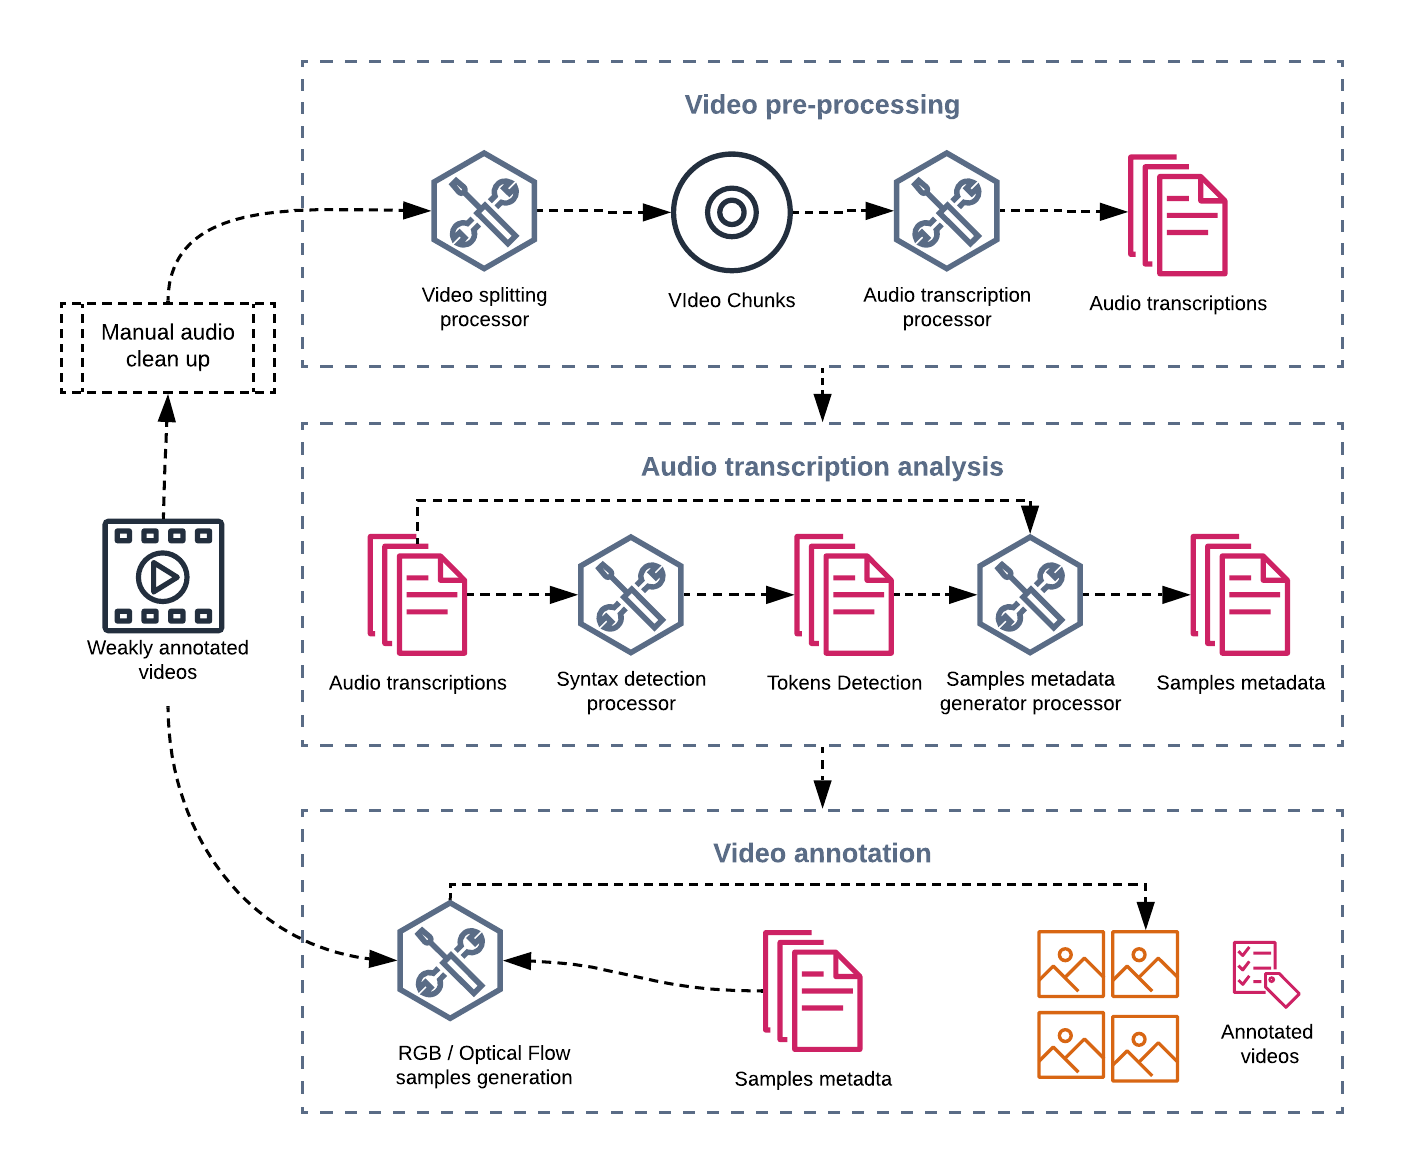
\includegraphics[width=\linewidth]{images/video-annotation-pipeline.png}
\caption{Video annotation process}
\label{fig:video-annotation-pipeline}
\end{figure}

\subsubsection{Manual Automatic Video Clean Up}\label{manual-video-cleanup}
The PSL recordings described on \ref{datasetdesc} contain a considerable amount of noise introduced during recording sessions. It makes difficult to easily find video intervals that clearly show a relation between signs emitted by the informant and the translation delivered by the translator. Noise factors are the following:
\begin{itemize}
	\item Multiple participants speaking during the session.
	\item Conversations between participants that are not relevant to emitted sings.
	\item High frequency of large silent periods.
\end{itemize}
A manual video cleanup process is required to find noise free video intervals. This process requires watching all the videos available at the PSL corpus for manually annotating the instant when an informant started emitting sings along with the instant when the translator delivered a translation, Table \ref{table:noise-free-video-segments} shows a manual annotation example.

The recordings show the informant in two alignments (centered and left), the manual video clean up process also stores the informant alignment, table \ref{table:informant-alignment} shows the two available alignments, we use the alignment annotation later in the process during the video frames extraction to create the labeled PSL dataset.

% Noise free video segment extract table
\begin{table}[!htb]
\captionsetup{font=footnotesize}
\centering
\begin{tabular}{lrrc}
\toprule
\multicolumn{1}{c}{\textbf{Video}} & 
	\multicolumn{1}{c}{\textbf{Start}} &
	\multicolumn{1}{c}{\textbf{End}} &
	\multicolumn{1}{c}{\textbf{Alignment}}\\
\midrule
\multirow{5}{7.5em}{\textbf{consultant-01-session-01-part-01.mp4}} & 00:30 & 00:55 & center\\
& 01:15 & 01:29 & center\\
& 00:53 & 01:07 & center\\
& 08:12 & 09:01 & center\\
\midrule
\multirow{5}{7.5em}{\textbf{consultant-02-session-01-part-01.mp4}} & 00:15 & 00:21 & center\\
& 00:15 & 00:21 & center\\
& 00:53 & 01:07 & center\\
& 02:43 & 02:47 & center\\
& 17:33 & 18:01 & left\\
\bottomrule
\end{tabular}
\captionsetup{font=footnotesize}
\caption{Noise free video segments extract} \label{table:noise-free-video-segments}
\end{table}

% Informat aligment
\begin{table}[!htb]
\captionsetup{font=footnotesize}
\centering
\begin{tabular}{cc}
\toprule
\multicolumn{1}{c}{\textbf{Center Aligned}} & 
	\multicolumn{1}{c}{\textbf{Left Aligned}}\\
\midrule
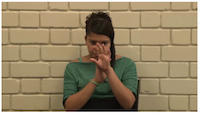
\includegraphics{images/informant-center-alignment.png}& 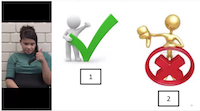
\includegraphics{images/informant-left-alignment.png}\\
\bottomrule
\end{tabular}
\caption{Informant Alignment} \label{table:informant-alignment}
\end{table}

\subsubsection{Video Pre-Processing}\label{video-pre-processing}
Non-annotated PSL videos require processing before any metadata can be extracted, we propose a sequence of pre-processing tasks that take advantage of the annotation generated on \ref{manual-video-cleanup}. A \textbf{video splitting processor} generates a set of video chunks using the \textit{ffmpeg} multimedia framework and stores produced video chunks in Amazon S3 for later usage. Audio within video chunks is then transcribed by an \textbf{audio transcription processor}, using the Amazon Transcription service, we selected the Amazon Transcription service because it provides an accurate mapping between audio participants and transcribed words along with useful metadata that describes the start and end time when words are pronounced by the translator. 

At the moment of writing this work Amazon Transcription service only supported Spain and US Spanish. This caused certain words that are specific for Peruvian Spanish not being fully recognized, in order to improve transcription accuracy we built a custom vocabulary containing Peruvian expressions which improved  Peruvian words recognition, for the matters of this work Peruvian words that remained unrecognized were omitted and not processed.

\subsubsection{Audio Transcription Analysis}\label{audio-transcription-analysis}
Audio transcription requires additional processing in order to produce useful information that leads to a successful PSL signs detection. Bag of Embedding Words (BoEW) is a widely used technique on Natural Language Processing tasks providing a easy and flexible way to list the most relevant words based on frequency. This work is focused on detecting nouns and numbers (our method is designed to be progressively improved to handle a wider set of PSL elements) assuming that nouns (numbers are a subset of nouns) suffer less variations in spoken Spanish than verbs, pronouns, adverbs and adjectives, and provide more semantic value than conjunctions, prepositions and interjections. 

\begin{table}[!htb]
\captionsetup{size=footnotesize}
\begin{tabular}{ p{16em} c}
\toprule
\multicolumn{1}{c}{\textbf{Token}} & 
	\multicolumn{1}{c}{\textbf{Frequency}}\\
\midrule
\textbf{pareja}&	40\\
\textbf{cosas}&	30\\
\textbf{cine}&	20\\
\textbf{noche}&	20\\
\textbf{terror}&	10\\
\textbf{parque}&	10\\
\textbf{casa}&	10\\
\textbf{montón}&	10\\
\textbf{apariciones}&	10\\
\textbf{fantasmas}&	10\\
\textbf{dos}&	10\\
\bottomrule
\end{tabular}
\caption{Most relevant tokens detection frequency in the PSL dataset} \label{tab:token-freq}
\end{table}

We used Amazon comprehend for text analysis, specifically the syntax detection functionality which will provide a comprehensive list of detected language elements along with a score from 0.0 to 1.0 indicating the detection accuracy, we have selected the ones that have at least a 0.8 accuracy score and omitted the rest, this process was automated using a \textbf{transcription detection processor} which uses BoEW to provide a list of most relevant nouns and numbers based on appearance frequency. Table \ref{tab:token-freq} shows a list of nouns and numbers and their frequencies in the PSL dataset.

Once a weighted list of nouns and numbers is generated a mapping showing when nouns and numbers appear in videos is required, moving forward called \textbf{Samples Metadata}. Table \ref{tab:token-video-mapping} shows mapping metadata extracted from PSL.

\subsubsection{Samples Generation}\label{samples-generation} 
Our method requires PSL elements to be represented as a set of RGB frames and a calculated Optical Flow using the Lucas-Kanade method, both representations are inputs of two different models as presented on \ref{nsdm}.

\textbf{Translation Delay Factor: } The difference in time between the instant when a sign is emitted and when a translation for that given sign is delivered is uncertain, we are calling that uncertainty \textit{the translation delay factor}, we are trying to approximate it using a constant value, we chose a three seconds translation delay factor assuming that most of the translations will occur between three seconds after a sign is emitted.

A \textbf{RGB Samples generation processor} uses samples metadata in combination with the translation delay factor to determine frames that represent a given PSL element. We use \textit{OpenCV} to extract frames and store them following a hierarchical folder structure (listing \ref{list:rgb-samples-folders}) that nSDm data loaders will use to feed data into the RGB branch in the nSDm model architecture \ref{nsdm-architecture} during training and testing.

An \textbf{Optical Flow Samples generation processor} uses video frames and the hierarchical folder structure generated by the RGB samples generation processor to calculate an Optical Flow representation for PSL elements and store them in a hierarchical folder structure that will also be used by the nSDm data loaders to feed the optical flow branch on the nSDm model architecture \ref{nsdm-architecture} during training and testing. We selected optical flow as a samples generation strategy due to its ability to represent movement traces from previous frames. It is particular useful for representing body movement patterns executed by informant while emitting a PSL sign. A PSL sign is made up of different body movements including: elbow, arms, neck, eyes, shoulders and hands, which are performed quickly, a way to detect movement traces between frames allows to generate a single image representation of all movement involved on a sign emission(Figure \ref{fig:opticalflow-two}). 

\begin{table}[!htb]
\captionsetup{font=footnotesize}
\centering
\begin{tabular}{ l p{10em} r r }
\toprule
\multicolumn{1}{c}{\textbf{Token}} & 
	\multicolumn{1}{c}{\textbf{Video}} &
	\multicolumn{1}{c}{\textbf{Start}} &
	\multicolumn{1}{c}{\textbf{End}}\\
\midrule
\textbf{cine}&	consultant-02-session-01-part-01-00.mp4&	4.19&	4.75\\
\textbf{cine}&	consultant-02-session-01-part-01-01.mp4&	1.19&	1.75\\
\textbf{terror}&	consultant-02-session-01-part-01-01.mp4&	3.82&	4.4\\
\textbf{parque}&	consultant-02-session-01-part-01-03.mp4&	8.97&	9.3\\
\textbf{casa}&	consultant-02-session-01-part-01-03.mp4&	10.12&	10.57\\
\textbf{pareja}&	consultant-02-session-01-part-01-04.mp4&	3.91&	4.36\\
\textbf{noche}&	consultant-02-session-01-part-01-04.mp4&	4.49&	4.92\\
\textbf{noche}&	consultant-02-session-01-part-01-04.mp4&	7.91&	8.2\\
\textbf{mont\'on}&	consultant-02-session-01-part-01-04.mp4&	8.5&	8.78\\
\textbf{cosas}&	consultant-02-session-01-part-01-04.mp4&	8.88&	9.38\\
\bottomrule
\end{tabular}
%\end{tabular}}
\caption{Shows metadata extacted from the PSL dataset: (1)\textit{Token} could be a noun or a number (2)\textit{Video Path} shows the video where the token was detected (3)\textit{Start Time} time when the token reproduction starts (4)\textit{End Time} time when the token reproduction ends.}
\label{tab:token-video-mapping}
\end{table}

\subsection{Novel Signs Detection Model (nSDm)}\label{nsdm}
We propose a novel model for signs detection that combine two neural networks architectures, a CNN and a RNN with the objective to learn visual features like edges, corners and ridges (CNN) and at the same time patterns learned from a time based series of inputs (RNN). CNN network receives optical flow inputs and the RNN branch receives RGB frames extracted from the labeled PSL dataset described in \ref{videoannot}.

For this work we selected the Tensorflow/Keras functional API for its ability to define combined models along with a versatile data extraction and transformation layer. More details and usage are provided in sections \ref{nsdm-architecture} and \ref{new-videos-testing}

Implementation details can be found at https://github.com/erichuizapucp/signs-recognition
\subsubsection{Architecture}\label{nsdm-architecture}
A series of models stacked in a composed architecture focused on learning visual and time series features using two network architecture flavors enforced with a flexible data input pipeline for data feeding as shown in Figure \ref{fig:ndsm-architecture}, transformation and normalization. 

The \textbf{Input pipeline} accesses the labeled PSL samples and applies transformations preparing the data for upper layers, transformations were applied to both optical flow and RGB frames, PSL samples were resized to be compliant with ImageNet pre-trained models using a 224 by 224 shape and three channels for color images, data augmentation transformation were not applied due to the nature of the experiment where samples were captured using similar light conditions and camera orientations, PSL samples were transformed to tensors and normalized to floats in the [0, 1] interval, finally the transformed and normalized versions of optical flow and RGB samples were tight together in a tensor structure along with the label for usage at upper layers.
\begin{table}[!htb]
\captionsetup{size=footnotesize}
\begin{tabular}{ p{16em} c}
\toprule
\multicolumn{1}{c}{\textbf{Hyper parameter}} & 
	\multicolumn{1}{c}{\textbf{Value}}\\
\midrule
\textbf{Learning Rate}&	0.001\\
\textbf{No Epochs}&	5\\
\textbf{No Steps per Epoch}&	5\\
\textbf{Batch Size}&	10\\
\textbf{Shuffle Buffer Size}&	50\\
\bottomrule
\end{tabular}
\caption{nSDm training hyper parameters} \label{tab:nSDm-hyperparams}
\end{table}

The \textbf{Wrapper Layer} wraps a CNN network designed for learning visual features from optical flow and a RNN network designed for learning features from series of video frames, the layer receives data from the input pipeline then splits it into optical flow and RGB samples and passes them to the CNN and RNN networks respectively. The logits produced are then concatenated and passed to the dense layer.

The dense layer uses a softmax activation function to convert logits into probabilities used for a correct sign classification. Hyper parameters used during the training process are listed on Table \ref{tab:nSDm-hyperparams}

\begin{figure}[hbt!]
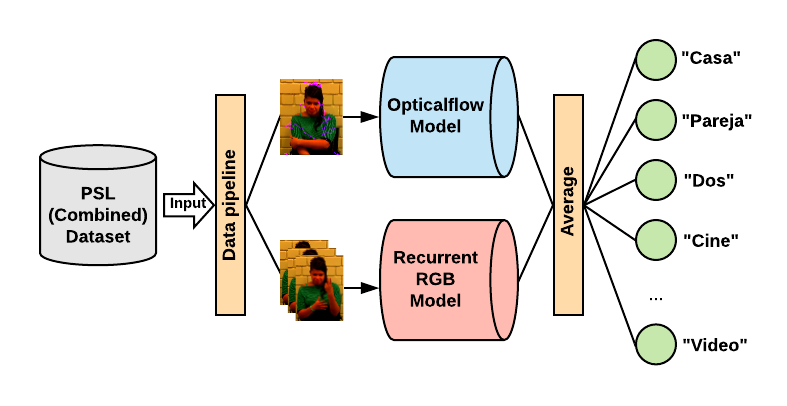
\includegraphics[width=\linewidth]{images/nsdm-model-architecture.png}
\caption{nSDm model architecture}
\label{fig:ndsm-architecture}
\end{figure}

The \textbf{Opticalflow model} described in Figure \ref{fig:opticalflow-architecture} receives decoded opticalflow samples, it uses a Resnet152 backbone pre-trained with ImageNet, we used a fine tuning transfer learning approach, the backbone produces a 7x7x2048 output that then is passed to a Global Average Pooling layer for obtaining a flattened output of 1x1x2048 which is then passed to a dense layer for logits computation.

\begin{figure}[hbt!]
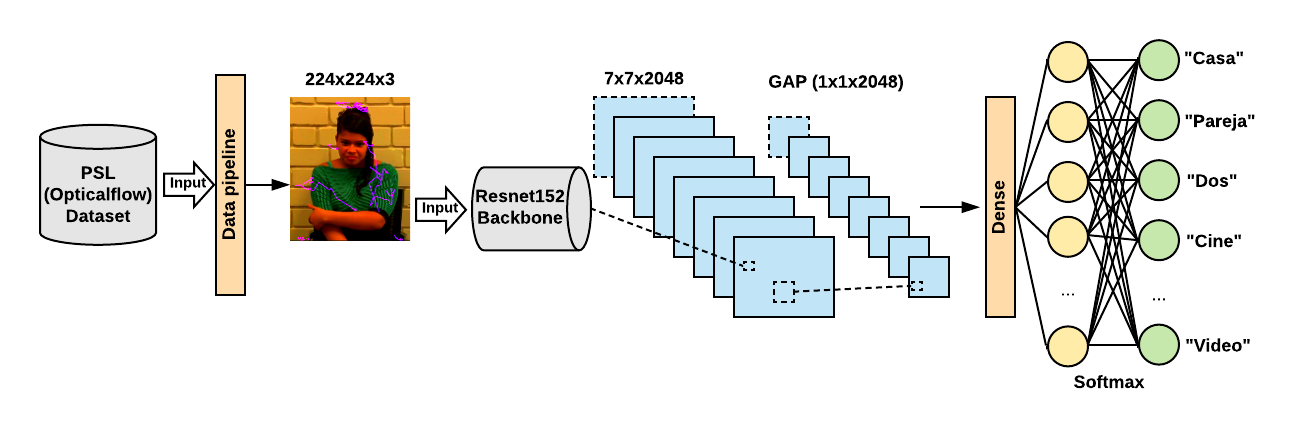
\includegraphics[width=\linewidth]{images/opticalflow-model-architecture.png}
\caption{Opticalflow model architecture}
\label{fig:opticalflow-architecture}
\end{figure}

The \textbf{Recurrent RGB model} described in Figure \ref{fig:rgb-architecture} receives a sequence of decoded video frames, it uses a \textit{many-to-one} architecture with LSTM cells that hold state of 2048 units length, the output produced by the recurrent layers is then passed to a dense layer for logits computation.

\begin{figure}[hbt!]
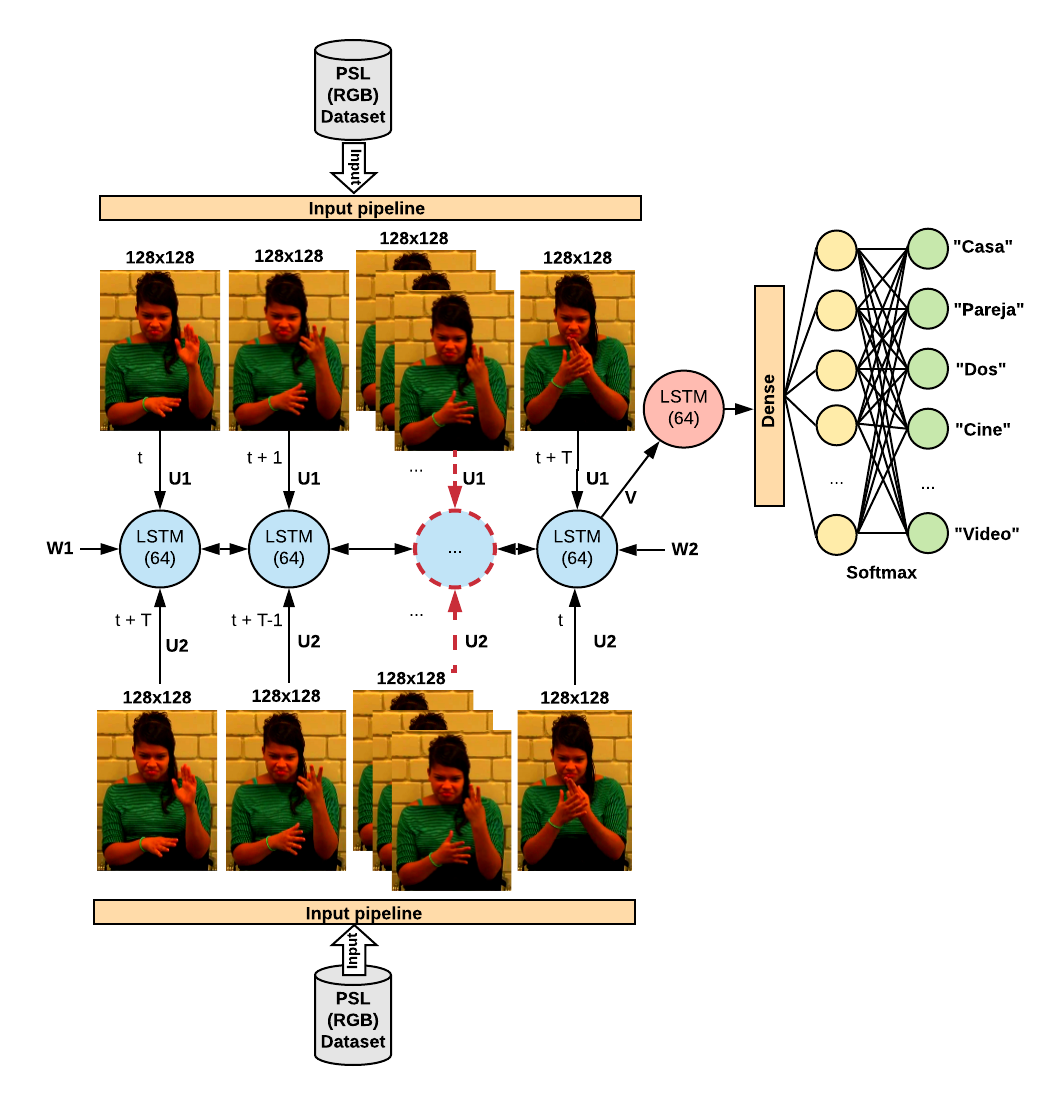
\includegraphics[width=\linewidth]{images/recurrent-rgb-model-architecture.png}
\caption{Recurrent RGB model architecture}
\label{fig:rgb-architecture}
\end{figure}

Logits produced by the opticalflow and recurrent RGB models are concatenated and then passed to a dense layer with a softmax activation function producing PSL signs detection probabilities.

\subsection{Sign detection testing}\label{new-videos-testing}
We selected videos for consultant 24 which will be described in \ref{datasetdesc} for testing nSDm (the model was not trained with consultant 24 videos), we proceed to extract RGB frames for video fragments of five seconds length moving ahead one second on each loop until the end of the video that way we can reduce the number of signs cut or incomplete between video fragments. Optical flow and RGB frames generators feed nSDm for detecting signs \ref{nsdm} present in the video fragment.

A software component called Video Updater uses video metadata produced by the RGB Frames Generator like start and end time in seconds and detected signs for annotating the video adding a mask that highlights detected signs. We used OpenCV for incorporating masks to test videos, Figure \ref{fig:video-testing-architecture} shows the signs detection testing architecture.
\begin{figure}[hbt!]
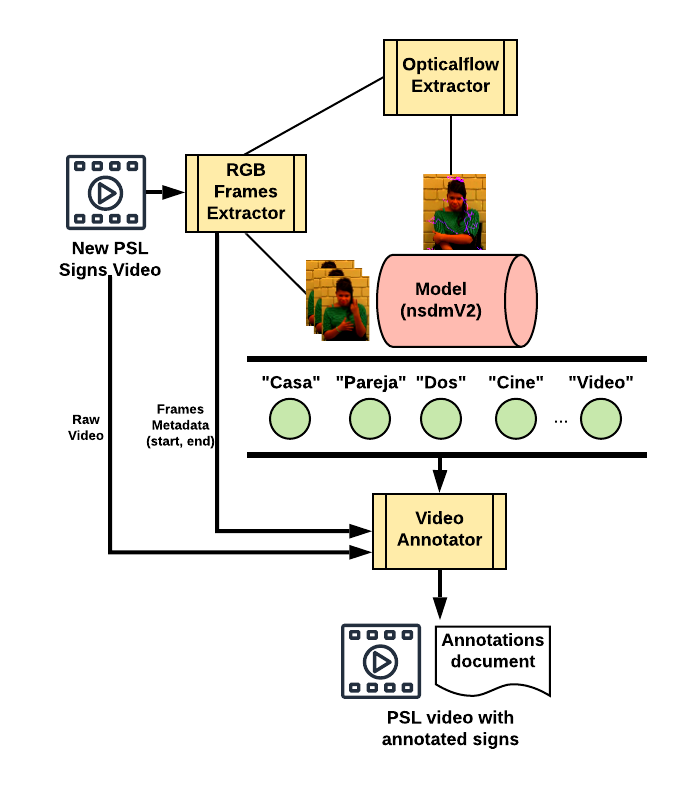
\includegraphics[width=\linewidth]{images/new-video-test-architecture.png}
\caption{Signs detection testing process architecture}
\label{fig:video-testing-architecture}
\end{figure}

\section{Experimentation}\label{experimentation}
\subsection{Dataset Description \cite{lsp_dataset}}\label{datasetdesc}
The PSL dataset was developed by the PUCP Grammar and Signs research group in 2014 and consists in a set of videos recorded during the interviews of 24 individuals, 12 male and 12 female informants, all of them are Lima Peru residents and reported to be born with a permanent deafness condition or acquired the condition before the acquisition of Spanish. 

The dataset consists in 718 video clips recorded with a ADR-CX220 SONY HD camera which included an embedded microphone. The camera focused only the informant but also recorded questions, instructions and translations.

The video clips were recorded in three sessions with the following participants: A coordinator, a PSL \cite{lsp_2015} translator and a informant.\\

\textbf{Recording Session 1}: A 45-60 minutes semi structured interview that included: Biographic information as well as habits, anecdotes, opinion about cultural subjects and elicitation of names, states and actions. 

\textbf{Recording Session 2}: The informant was presented with a set of 55 cards describing actions and were asked to choose a set of them in order to build a coherent story that was subsequently told by the informant.

\textbf{Recording Session 3}: A PSL \cite{lsp_2015} conversation facilitated by the coordinator happening between the informant and the translator.\\

During all the sessions a PSL \cite{lsp_2015} translator performs a translation after a word or phrase is completed.

\subsection{Video Annotation Results}\label{video-annotation-results}
The video annotation pipeline described on \ref{videoannot} produced an annotated PSL dataset suitable for using it in a supervised learning experiment. The annotated dataset is divided in two main parts (RGB and Optical Flow samples)

\textbf{RGB Samples folder structure} is a hierarchical folder structure where each detected noun or number is represented as a first level folder, all instances of a detected sign received an identifier which is an auto incremental integer, detected instances represent the second level folders, detected signs video represent the third level, Figure \ref{fig:rgb-two}.
\begin{lstlisting}[caption=RGB Samples Folder Structure example, basicstyle=\ttfamily\small]
L1:dos
	L2:1
		L3:rgb-frame01.jpg
		L3:rgb-frame02.jpg
		L3:rgb-frame03.jpg
		...
		L3:rgb-frame08.jpg
L1:cine
	L2:1
		L3:rgb-frame01.jpg
		L3:rgb-frame02.jpg
		L3:rgb-frame03.jpg
		...
		L3:rgb-frame15.jpg
	L2:2
		L3:rgb-frame01.jpg
		L3:rgb-frame02.jpg
		L3:rgb-frame03.jpg
		...
		L3:rgb-frame11.jpg
\end{lstlisting}\label{list:rgb-samples-folders}

\begin{figure}[hbt!]
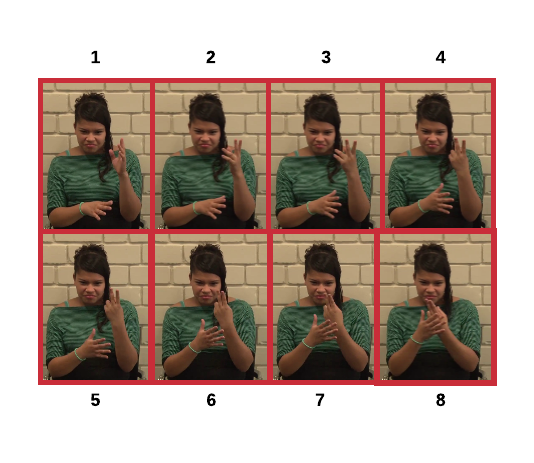
\includegraphics[width=\linewidth]{images/dos-rgb-frames.png}
\caption{PSL number "Two" RGB representation}
\label{fig:rgb-two}
\end{figure}

\textbf{Optical Flow samples folder structure} is a hierarchical folder structure based on the RGB samples folder structure, it is a more simple based on two levels instead of three, the nature of Optical Flow of tracing movement between frames allow to produce a single image for each detected PSL element instance (listing \ref{list:opticalflow-samples-folders}), Figure \ref{fig:opticalflow-two} shows an example of an optical flow generated sample
\begin{lstlisting}[caption=Optical Flow Samples Folder Structure example, basicstyle=\ttfamily\small]
L1:dos
	L2:oflow-dos-01.jpg
L1:cine
	L2:oflow-cine-01.jpg
	L2:oflow-cine-02.jpg
\end{lstlisting}\label{list:opticalflow-samples-folders}
\begin{figure}[hbt!]
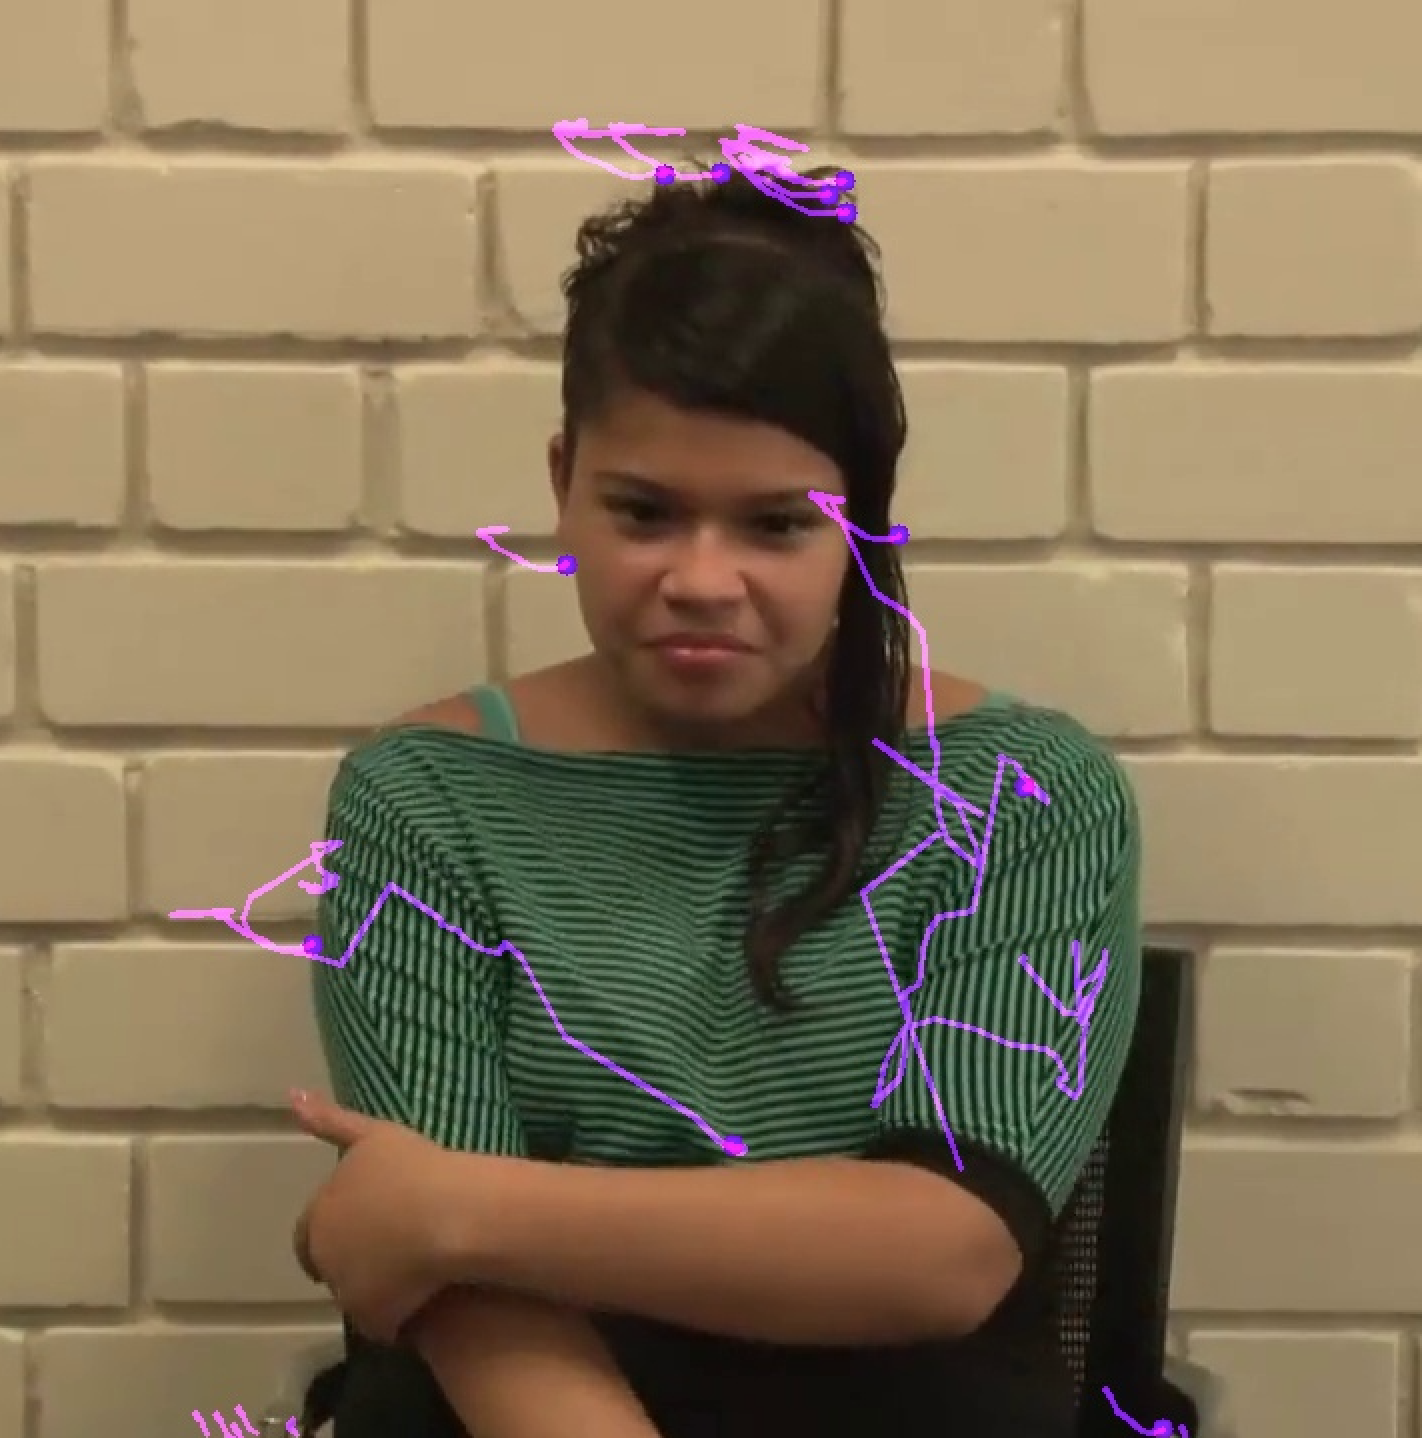
\includegraphics[width=\linewidth]{images/dos-opticalflow.jpg}
\caption{PSL number "Two" OpticalFlow representation}
\label{fig:opticalflow-two}
\end{figure}

\subsection{Sign detection results}
We trained nSDm with the train PSL dataset and validated it with the validation PSL dataset, preliminary we trained the model only for five epochs obtaining the results in Table \ref{tab:signs-detection-results}
% Sign detection results
\begin{table}[!htb]
\captionsetup{font=footnotesize}
\centering
\begin{tabular}{ p{16em} c }
\toprule
\multicolumn{1}{c}{\textbf{Epoch}} & 
	\multicolumn{1}{c}{\textbf{AUC}}\\
\midrule
\textbf{Epoch 1}&	0.0368\\
\textbf{Epoch 2}&	0.5994\\
\textbf{Epoch 3}&	0.0412\\
\textbf{Epoch 4}&	0.0703\\
\textbf{Epoch 5}&	0.0680\\
\bottomrule
\end{tabular}
\caption{Shows results of training nSDm with the labeled PSL dataset: (1)\textit{Epoch} identifies the epoch in in the training process (2)\textit{AUC} area under the precision-recall curve (3)\textit{Precision} obtained precision (4)\textit{Recall} obtained recall.}
\label{tab:signs-detection-results}
\end{table}

\section{Conclusion}\label{conclusion}
\begin{enumerate}[i]
\item The ability of detecting recording sessions participants and a mapping between transcripted words and video instants are necessary for a correct video annotation because it allows differentiating PSL translations from other recording session transcriptions.
\item Video annotation requires a considerable amount of manual work, even though several steps in the proposed video annotation pipeline can be automated e.g. video splitting, audio transcription, syntax detection and metadata generation, pre video annotation and post verification steps are executed manually.
\item Post samples verification steps are required due to the \textit{Delay Factor}, frames not related to a sign are deleted to improve the labeled PSL dataset quality.
\item Using optical flow for movement pattern representation allow capturing all actions and movements executed by a PSL consultant.
\item A CNN can be trained with optical flow samples to recognize human actions making possible to learn PSL signs movement patterns.
\item RGB video frames extracted from video fragments can be used to train a RNN for learning human actions, the network learns movement sequences between frames making possible to learn PSL signs movement sequences.
\item Combining a CNN and a RNN in a composite model improves signs detection performance, while CNNs learns visual features in optical flow samples RNNs learns sequences of actions, networks outputs can be pondered for training a better classifier.
\item The area under the precision-recall curve allow measuring how well is nSDm detecting because it summarizes the trade-off between the true positive signs rate and the predicted signs.
\end{enumerate}

\bibliographystyle{ieeetr}
\bibliography{References}


\end{document}
